\section{Instance Initialization and
destruction}\label{instance-initialization-and-destruction}

A new version of the text file editor (\passthrough{\lstinline!tfe!})
will be made in this section and the following four sections. It is
\passthrough{\lstinline!tfe5!}. There are many changes from the prior
version. They are located in two directories, src/tfe5 and
src/tfetextview.

\subsection{Encapsulation}\label{encapsulation}

We've divided C source file into two parts. But it is not enough in
terms of encapsulation.

\begin{itemize}
\tightlist
\item
  \passthrough{\lstinline!tfe.c!} includes everything other than
  TfeTextView. It should be divided into at least two parts,
  \passthrough{\lstinline!tfeapplication.c!} and
  \passthrough{\lstinline!tfenotebook.c!}.
\item
  Header files also need to be organized.
\end{itemize}

However, first of all, I'd like to focus on the object TfeTextView. It
is a child object of GtkTextView and has a new member
\passthrough{\lstinline!file!} in it. The important thing is to manage
the Gfile object pointed by \passthrough{\lstinline!file!}.

\begin{itemize}
\tightlist
\item
  What is necessary to GFile when creating (or initializing)
  TfeTextView?
\item
  What is necessary to GFile when destructing TfeTextView?
\item
  Should TfeTextView read/write a file by itself or not?
\item
  How it communicates with objects outside?
\end{itemize}

You need to know at least class, instance and signals before thinking
about them. I will explain them in this section and the next section.
After that I will explain:

\begin{itemize}
\tightlist
\item
  Organizing functions.
\item
  How to use GtkFileDialog. It is a new class made in the version 4.10
  and replaces GtkFileChooserDialog.
\end{itemize}

\subsection{GObject and its children}\label{gobject-and-its-children}

GObject and its children are objects, which have both class and object C
structures. First, think about instances. An instance is memories which
has the object structure. The following is the structure of TfeTextView.

\begin{lstlisting}[language=C]
/* This typedef statement is automatically generated by the macro G_DECLARE_FINAL_TYPE */
typedef struct _TfeTextView TfeTextView;

struct _TfeTextView {
  GtkTextView parent;
  GFile *file;
};
\end{lstlisting}

The members of the structure are:

\begin{itemize}
\tightlist
\item
  The member \passthrough{\lstinline!parent!} is a GtkTextView C
  structure. It is declared in \passthrough{\lstinline!gtktextview.h!}.
  GtkTextView is the parent of TfeTextView.
\item
  The member \passthrough{\lstinline!file!} is a pointer to a GFile. It
  can be NULL if the TfeTextView instance has no file. The most common
  case is that the instance is newly created.
\end{itemize}

You can find the declaration of the structures of the ancestors in the
source files in GTK or GLib. The following is extracted from the source
files (not exactly the same).

\begin{lstlisting}[language=C]
typedef struct _GObject GObject;
typedef struct _GObject GInitiallyUnowned;
struct  _GObject
{
  GTypeInstance  g_type_instance;
  volatile guint ref_count;
  GData         *qdata;
};

typedef struct _GtkWidget GtkWidget;
struct _GtkWidget
{
  GInitiallyUnowned parent_instance;
  GtkWidgetPrivate *priv;
};

typedef struct _GtkTextView GtkTextView;
struct _GtkTextView
{
  GtkWidget parent_instance;
  GtkTextViewPrivate *priv;
};
\end{lstlisting}

In each structure, its parent is declared at the top of the members. So,
all the ancestors are included in the child object. The structure of
\passthrough{\lstinline!TfeTextView!} is like the following diagram.

\begin{figure}
\centering
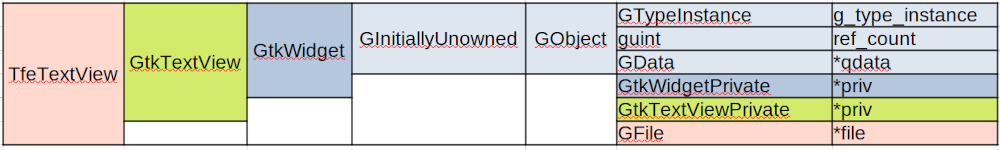
\includegraphics[width=14.39cm,height=2.16cm]{../image/TfeTextView.png}
\caption{The structure of the instance TfeTextView}
\end{figure}

Derivable classes (ancestor classes) have their own private data area
which are not included by the structure above. For example, GtkWidget
has GtkWidgetPrivate (C structure) for its private data.

Notice declarations are not definitions. So, no memories are allocated
when C structures are declared. Memories are allocated to them from the
heap area when the \passthrough{\lstinline!tfe\_text\_view\_new!}
function is called. At the same time, the ancestors' private area
allocated for the TfeTetView. They are hidden from TfeTextView and it
can't access to them directly. The created memory is called instance.
When a TfeTextView instance is created, it is given three data area.

\begin{itemize}
\tightlist
\item
  The instance (C structure).
\item
  GtkWidgetPrivate structure.
\item
  GtkTextViewPrivate structure.
\end{itemize}

TfeTextView functions can access to its instance only. The
GtkWidgetPrivate and GtkTextViewPrivate are used by the ancestors'
functions. See the following example.

\begin{lstlisting}[language=C]
GtkWidget *tv = tfe_text_view_new ();
GtkTextBuffer *buffer = gtk_text_view_get_buffer (GTK_TEXT_VIEW (tv));
\end{lstlisting}

The parent's function
\passthrough{\lstinline!gtk\_text\_view\_get\_buffer!} accesses the
GtkTextViewPrivate data (owned by \passthrough{\lstinline!tv!}). There
is a pointer, which points the GtkBuffer, in the private area and the
function returns the pointer. (Actual behavior is a bit more
complicated.)

TfeTextView instances inherit the ancestors functions like this.

A TfeTextView instance is created every time the
\passthrough{\lstinline!tfe\_text\_view\_new!} function is called.
Therefore, multiple TfeTextView instances can exist.

\subsection{Initialization of TfeTextView
instances}\label{initialization-of-tfetextview-instances}

The function \passthrough{\lstinline!tfe\_text\_view\_new!} creates a
new TfeTextView instance.

\begin{lstlisting}[language=C, numbers=left]
GtkWidget *
tfe_text_view_new (void) {
  return GTK_WIDGET (g_object_new (TFE_TYPE_TEXT_VIEW, "wrap-mode", GTK_WRAP_WORD_CHAR, NULL));
}
\end{lstlisting}

When this function is invoked, a TfeTextView instance is created and
initialized. The initialization process is as follows.

\begin{enumerate}
\def\labelenumi{\arabic{enumi}.}
\tightlist
\item
  When the instance is created, GtkWidgetPrivate and GtkTextViewPrivate
  structures are also created
\item
  Initializes GObject (GInitiallyUnowned) part in the TfeTextView
  instance.
\item
  Initializes GtkWidget part (the first \passthrough{\lstinline!priv!})
  in the TfeTextView instance and GtkWidgetPrivate structure.
\item
  Initializes GtkTextView part (the second
  \passthrough{\lstinline!priv!}) in the TfeTextView instance and
  GtkTextViewPrivate structure.
\item
  Initializes TfeTextView part (\passthrough{\lstinline!file!}) in the
  TfeTextView instance.
\end{enumerate}

The step two through four is done by
\passthrough{\lstinline!g\_object\_init!},
\passthrough{\lstinline!gtk\_widget\_init!} and
\passthrough{\lstinline!gtk\_text\_view\_init!}. They are called by the
system automatically and you don't need to care about them. Step five is
done by the function \passthrough{\lstinline!tfe\_text\_view\_init!} in
\passthrough{\lstinline!tfetextview.c!}.

\begin{lstlisting}[language=C, numbers=left]
static void
tfe_text_view_init (TfeTextView *tv) {
  tv->file = NULL;
}
\end{lstlisting}

This function just initializes \passthrough{\lstinline!tv->file!} to be
\passthrough{\lstinline!NULL!}.

\subsection{Functions and Classes}\label{functions-and-classes}

In Gtk, all objects derived from GObject have classes and instances (but
abstract objects have only classes). Instances are memory of C
structure, which are described in the previous two subsections. Each
object can have more than one instance. Those instances have the same
structure. Instances just have data. Therefore, it doesn't define
object's behavior. We need at least two things. One is functions and the
other is class methods.

The latest GTK 4 document classifies functions into a constructor,
functions and instance methods.

\begin{itemize}
\tightlist
\item
  constructors: Their name are always
  \passthrough{\lstinline!gtk\_(objectname)\_new!}. They create the
  objects.
\item
  functions: Their first parameter (argument) is \emph{NOT} the
  instance. Usually functions are utility functions for the class.
\item
  instance methods: Their first parameter (argument) is the instance.
  They do some task for the specific instance.
\end{itemize}

This tutorial uses \passthrough{\lstinline!functions!} in two ways,
broad or narrow sense.

You've already seen many functions. For example,

\begin{itemize}
\tightlist
\item
  \passthrough{\lstinline!TfeTextView *tfe\_text\_view\_new (void);!} is
  a function (constructor) to create a TfeTextView instance.
\item
  \passthrough{\lstinline!GtkTextBuffer *gtk\_text\_view\_get\_buffer (GtkTextView *textview)!}
  is a function (instance method) to get a GtkTextBuffer from
  GtkTextView.
\end{itemize}

Functions are public, which means that they are expected to be used by
other objects. They are similar to public methods in object oriented
languages.

Class (C structure) mainly consists of pointers to C functions. They are
called \emph{class methods} and used by the object itself or its
descendant objects. For example, GObject class is declared in
\passthrough{\lstinline!gobject.h!} in GLib source files.

\begin{lstlisting}[language=C, numbers=left]
typedef struct _GObjectClass             GObjectClass;
typedef struct _GObjectClass             GInitiallyUnownedClass;

struct  _GObjectClass
{
  GTypeClass   g_type_class;

  /*< private >*/
  GSList      *construct_properties;

  /*< public >*/
  /* seldom overridden */
  GObject*   (*constructor)     (GType                  type,
                                 guint                  n_construct_properties,
                                 GObjectConstructParam *construct_properties);
  /* overridable methods */
  void       (*set_property)        (GObject        *object,
                                         guint           property_id,
                                         const GValue   *value,
                                         GParamSpec     *pspec);
  void       (*get_property)        (GObject        *object,
                                         guint           property_id,
                                         GValue         *value,
                                         GParamSpec     *pspec);
  void       (*dispose)         (GObject        *object);
  void       (*finalize)        (GObject        *object);
  /* seldom overridden */
  void       (*dispatch_properties_changed) (GObject      *object,
                         guint     n_pspecs,
                         GParamSpec  **pspecs);
  /* signals */
  void       (*notify)          (GObject    *object,
                     GParamSpec *pspec);

  /* called when done constructing */
  void       (*constructed)     (GObject    *object);

  /*< private >*/
  gsize     flags;

  gsize         n_construct_properties;

  gpointer pspecs;
  gsize n_pspecs;

  /* padding */
  gpointer  pdummy[3];
};
\end{lstlisting}

There's a pointer to the function \passthrough{\lstinline!dispose!} in
line 25.

\begin{lstlisting}[language=C]
void (*dispose) (GObject *object);
\end{lstlisting}

The declaration is a bit complicated. The asterisk before the identifier
\passthrough{\lstinline!dispose!} means pointer. So, the pointer
\passthrough{\lstinline!dispose!} points to a function which has one
parameter, which points a GObject structure, and returns no value. In
the same way, line 26 says \passthrough{\lstinline!finalize!} is a
pointer to the function which has one parameter, which points a GObject
structure, and returns no value.

\begin{lstlisting}[language=C]
void (*finalize) (GObject *object);
\end{lstlisting}

Look at the declaration of \passthrough{\lstinline!\_GObjectClass!} so
that you would find that most of the members are pointers to functions.

\begin{itemize}
\tightlist
\item
  13: A function pointed by \passthrough{\lstinline!constructor!} is
  called when the instance is created. It completes the initialization
  of the instance.
\item
  25: A function pointed by \passthrough{\lstinline!dispose!} is called
  when the instance destructs itself. Destruction process is divided
  into two phases. The first one is called disposing. In this phase, the
  instance releases all the references to other instances. The second
  phase is finalizing.
\item
  26: A function pointed by \passthrough{\lstinline!finalize!} finishes
  the destruction process.
\item
  The other pointers point to functions which are called while the
  instance lives.
\end{itemize}

These functions are called class methods. The methods are open to its
descendants. But not open to the objects which are not the descendants.

\subsection{TfeTextView class}\label{tfetextview-class}

TfeTextView class is a structure and it includes all its ancestors'
classes in it. Therefore, classes have similar hierarchy to instances.

\begin{lstlisting}
GObjectClass (GInitiallyUnownedClass) -- GtkWidgetClass -- GtkTextViewClass -- TfeTextViewClass
\end{lstlisting}

The following is extracted from the source codes (not exactly the same).

\begin{lstlisting}[language=C, numbers=left]
struct _GtkWidgetClass
{
  GInitiallyUnownedClass parent_class;

  /*< public >*/

  /* basics */
  void (* show)                (GtkWidget        *widget);
  void (* hide)                (GtkWidget        *widget);
  void (* map)                 (GtkWidget        *widget);
  void (* unmap)               (GtkWidget        *widget);
  void (* realize)             (GtkWidget        *widget);
  void (* unrealize)           (GtkWidget        *widget);
  void (* root)                (GtkWidget        *widget);
  void (* unroot)              (GtkWidget        *widget);
  void (* size_allocate)       (GtkWidget           *widget,
                                int                  width,
                                int                  height,
                                int                  baseline);
  void (* state_flags_changed) (GtkWidget        *widget,
                                GtkStateFlags     previous_state_flags);
  void (* direction_changed)   (GtkWidget        *widget,
                                GtkTextDirection  previous_direction);

  /* size requests */
  GtkSizeRequestMode (* get_request_mode)               (GtkWidget      *widget);
  void              (* measure) (GtkWidget      *widget,
                                 GtkOrientation  orientation,
                                 int             for_size,
                                 int            *minimum,
                                 int            *natural,
                                 int            *minimum_baseline,
                                 int            *natural_baseline);

  /* Mnemonics */
  gboolean (* mnemonic_activate)        (GtkWidget           *widget,
                                         gboolean             group_cycling);

  /* explicit focus */
  gboolean (* grab_focus)               (GtkWidget           *widget);
  gboolean (* focus)                    (GtkWidget           *widget,
                                         GtkDirectionType     direction);
  void     (* set_focus_child)          (GtkWidget           *widget,
                                         GtkWidget           *child);

  /* keyboard navigation */
  void     (* move_focus)               (GtkWidget           *widget,
                                         GtkDirectionType     direction);
  gboolean (* keynav_failed)            (GtkWidget           *widget,
                                         GtkDirectionType     direction);

  gboolean     (* query_tooltip)      (GtkWidget  *widget,
                                       int         x,
                                       int         y,
                                       gboolean    keyboard_tooltip,
                                       GtkTooltip *tooltip);

  void         (* compute_expand)     (GtkWidget  *widget,
                                       gboolean   *hexpand_p,
                                       gboolean   *vexpand_p);

  void         (* css_changed)                 (GtkWidget            *widget,
                                                GtkCssStyleChange    *change);

  void         (* system_setting_changed)      (GtkWidget            *widget,
                                                GtkSystemSetting      settings);

  void         (* snapshot)                    (GtkWidget            *widget,
                                                GtkSnapshot          *snapshot);

  gboolean     (* contains)                    (GtkWidget *widget,
                                                double     x,
                                                double     y);

  /*< private >*/

  GtkWidgetClassPrivate *priv;

  gpointer padding[8];
};

struct _GtkTextViewClass
{
  GtkWidgetClass parent_class;

  /*< public >*/

  void (* move_cursor)           (GtkTextView      *text_view,
                                  GtkMovementStep   step,
                                  int               count,
                                  gboolean          extend_selection);
  void (* set_anchor)            (GtkTextView      *text_view);
  void (* insert_at_cursor)      (GtkTextView      *text_view,
                                  const char       *str);
  void (* delete_from_cursor)    (GtkTextView      *text_view,
                                  GtkDeleteType     type,
                                  int               count);
  void (* backspace)             (GtkTextView      *text_view);
  void (* cut_clipboard)         (GtkTextView      *text_view);
  void (* copy_clipboard)        (GtkTextView      *text_view);
  void (* paste_clipboard)       (GtkTextView      *text_view);
  void (* toggle_overwrite)      (GtkTextView      *text_view);
  GtkTextBuffer * (* create_buffer) (GtkTextView   *text_view);
  void (* snapshot_layer)        (GtkTextView      *text_view,
                      GtkTextViewLayer  layer,
                      GtkSnapshot      *snapshot);
  gboolean (* extend_selection)  (GtkTextView            *text_view,
                                  GtkTextExtendSelection  granularity,
                                  const GtkTextIter      *location,
                                  GtkTextIter            *start,
                                  GtkTextIter            *end);
  void (* insert_emoji)          (GtkTextView      *text_view);

  /*< private >*/

  gpointer padding[8];
};

/* The following definition is generated by the macro G_DECLARE_FINAL_TYPE */
typedef struct {
  GtkTextView parent_class;
} TfeTextViewClass;
\end{lstlisting}

\begin{itemize}
\tightlist
\item
  120-122: This three lines are generated by the macro
  \passthrough{\lstinline!G\_DECLARE\_FINAL\_TYPE!}. So, they are not
  written in either \passthrough{\lstinline!tfe\_text\_view.h!} or
  \passthrough{\lstinline!tfe\_text\_view.c!}.
\item
  3, 84, 121: Each class has its parent class at the first member of its
  structure. It is the same as instance structures.
\item
  Class members in ancestors are open to the descendant class. So, they
  can be changed in
  \passthrough{\lstinline!tfe\_text\_view\_class\_init!} function. For
  example, the \passthrough{\lstinline!dispose!} pointer in GObjectClass
  will be overridden later in
  \passthrough{\lstinline!tfe\_text\_view\_class\_init!}. (Override is
  an object oriented programming terminology. Override is rewriting
  ancestors' class methods in the descendant class.)
\item
  Some class methods are often overridden.
  \passthrough{\lstinline!set\_property!},
  \passthrough{\lstinline!get\_property!},
  \passthrough{\lstinline!dispose!}, \passthrough{\lstinline!finalize!}
  and \passthrough{\lstinline!constructed!} are such methods.
\end{itemize}

TfeTextViewClass includes its ancestors' class in it. It is illustrated
in the following diagram.

\begin{figure}
\centering
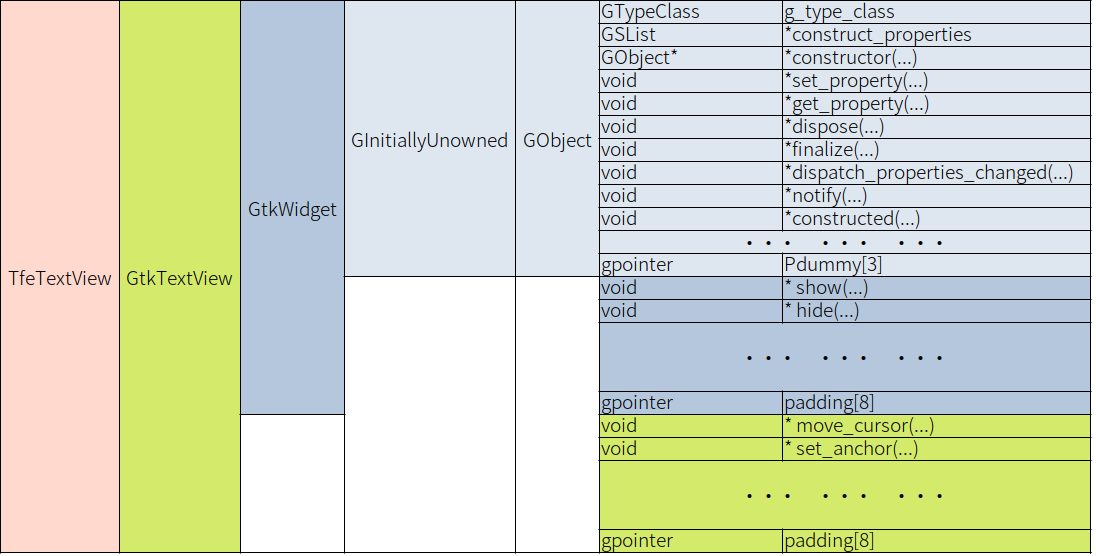
\includegraphics[width=16.02cm,height=8.34cm]{../image/TfeTextViewClass.png}
\caption{The structure of TfeTextView Class}
\end{figure}

\subsection{Destruction of
TfeTextView}\label{destruction-of-tfetextview}

Every Object derived from GObject has a reference count. If an object A
refers to an object B, then A keeps a pointer to B in A and at the same
time increases the reference count of B by one with the function
\passthrough{\lstinline!g\_object\_ref (B)!}. If A doesn't need B any
longer, A discards the pointer to B (usually it is done by assigning
NULL to the pointer) and decreases the reference count of B by one with
the function \passthrough{\lstinline!g\_object\_unref (B)!}.

If two objects A and B refer to C, then the reference count of C is two.
If A no longer needs C, A discards the pointer to C and decreases the
reference count in C by one. Now the reference count of C is one. In the
same way, if B no longer needs C, B discards the pointer to C and
decreases the reference count in C by one. At this moment, no object
refers to C and the reference count of C is zero. This means C is no
longer useful. Then C destructs itself and finally the memories
allocated to C is freed.

\begin{figure}
\centering
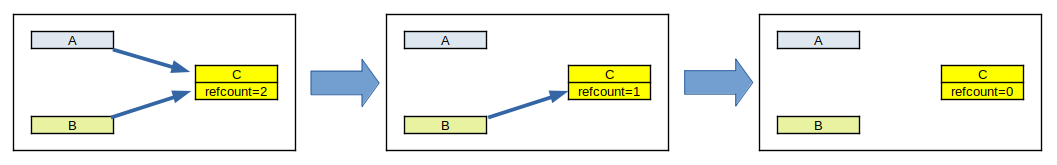
\includegraphics[width=15.855cm,height=2.475cm]{../image/refcount.png}
\caption{Reference count of B}
\end{figure}

The idea above is based on an assumption that an object referred by
nothing has reference count of zero. When the reference count drops to
zero, the object starts its destruction process. The destruction process
is split into two phases: disposing and finalizing. In the disposing
process, the object invokes the function pointed by
\passthrough{\lstinline!dispose!} in its class to release all references
to other instances. After that, it invokes the function pointed by
\passthrough{\lstinline!finalize!} in its class to complete the
destruction process.

In the destruction process, TfeTextView needs to unref the GFile pointed
by \passthrough{\lstinline!tv->file!}. You must write the dispose
handler \passthrough{\lstinline!tfe\_text\_view\_dispose!}.

\begin{lstlisting}[language=C, numbers=left]
static void
tfe_text_view_dispose (GObject *gobject) {
  TfeTextView *tv = TFE_TEXT_VIEW (gobject);

  if (G_IS_FILE (tv->file))
    g_clear_object (&tv->file);

  G_OBJECT_CLASS (tfe_text_view_parent_class)->dispose (gobject);
}
\end{lstlisting}

\begin{itemize}
\tightlist
\item
  5,6: If \passthrough{\lstinline!tv->file!} points a GFile, it
  decreases the reference count of the GFile instance. The function
  \passthrough{\lstinline!g\_clear\_object!} decreases the reference
  count and assigns NULL to \passthrough{\lstinline!tv->file!}. In
  dispose handlers, we usually use
  \passthrough{\lstinline!g\_clear\_object!} rather than
  \passthrough{\lstinline!g\_object\_unref!}.
\item
  8: invokes parent's dispose handler. (This will be explained later.)
\end{itemize}

In the disposing process, the object uses the pointer in its class to
call the handler. Therefore,
\passthrough{\lstinline!tfe\_text\_view\_dispose!} needs to be
registered in the class when the TfeTextView class is initialized. The
function \passthrough{\lstinline!tfe\_text\_view\_class\_init!} is the
class initialization function and it is declared in the
\passthrough{\lstinline!G\_DEFINE\_TYPE!} macro expansion.

\begin{lstlisting}[language=C]
static void
tfe_text_view_class_init (TfeTextViewClass *class) {
  GObjectClass *object_class = G_OBJECT_CLASS (class);

  object_class->dispose = tfe_text_view_dispose;
}
\end{lstlisting}

Each ancestors' class has been created before TfeTextViewClass is
created. Therefore, there are four classes and each class has a pointer
to each dispose handler. Look at the following diagram. There are four
classes -- GObjectClass (GInitiallyUnownedClass), GtkWidgetClass,
GtkTextViewClass and TfeTextViewClass. Each class has its own dispose
handler -- \passthrough{\lstinline!dh1!}, \passthrough{\lstinline!dh2!},
\passthrough{\lstinline!dh3!} and
\passthrough{\lstinline!tfe\_text\_view\_dispose!}.

\begin{figure}
\centering
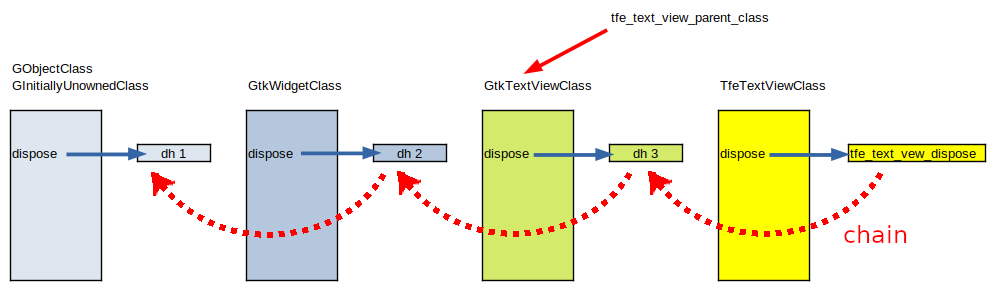
\includegraphics[width=14.925cm,height=4.455cm]{../image/dispose_handler.png}
\caption{dispose handlers}
\end{figure}

Now, look at the \passthrough{\lstinline!tfe\_text\_view\_dispose!}
program above. It first releases the reference to GFile object pointed
by \passthrough{\lstinline!tv->file!}. Then it invokes its parent's
dispose handler in line 8.

\begin{lstlisting}[language=C]
G_OBJECT_CLASS (tfe_text_view_parent_class)->dispose (gobject);
\end{lstlisting}

A variable \passthrough{\lstinline!tfe\_text\_view\_parent\_class!},
which is made by \passthrough{\lstinline!G\_DEFINE\_FINAL\_TYPE!} macro,
is a pointer that points the parent object class. The variable
\passthrough{\lstinline!gobject!} is a pointer to TfeTextView instance
which is casted as a GObject instance. Therefore,
\passthrough{\lstinline!G\_OBJECT\_CLASS (tfe\_text\_view\_parent\_class)->dispose!}
points the handler \passthrough{\lstinline!dh3!} in the diagram above.
The statement
\passthrough{\lstinline!G\_OBJECT\_CLASS (tfe\_text\_view\_parent\_class)->dispose (gobject)!}
is the same as \passthrough{\lstinline!dh3 (gobject)!}, which means it
releases all the reference to the other instances in the
GtkTextViewPrivate in the TfeTextView instance. After that,
\passthrough{\lstinline!dh3!} calls \passthrough{\lstinline!dh2!}, and
\passthrough{\lstinline!dh2!} calls \passthrough{\lstinline!dh1!}.
Finally all the references are released.
